\section{点与曲线}
\label{sec:mfd-points-curves}

流形是一个整体空间，它的元素是点。在欧氏空间中，点与它的坐标几乎不加区分；在流形上，坐标只是某张局部地图对点的记录，换一张图记录就变。先弄清哪些运算属于点、哪些只属于坐标，再用参数曲线描述点随参数的连续变化。

\subsection{点的坐标表示}
\label{sec:mfd-point-coordinates}

取球面上的点$p=(0,\tfrac35,\tfrac45)$，它就是图~\ref{fig:mfd-stereographic}(b)中的那一点。按式~\eqref{eq:mfd-stereographic-north}，分母是$1-\tfrac45=\tfrac15$，所以北极图坐标是
\[
\sigma_N(p)=\frac{(0,\tfrac35)}{1/5}=(0,3).
\]
按式~\eqref{eq:mfd-stereographic-south}，分母是$1+\tfrac45=\tfrac95$，所以南极图坐标是
\[
\sigma_S(p)=\frac{(0,\tfrac35)}{9/5}=(0,\tfrac13).
\]
两组数不同，记录的是同一个点。代入转移映射\eqref{eq:mfd-stereographic-transition}核对：$\tau(0,3)=(0,3)/9=(0,\tfrac13)$，正好对上。

\paragraph{坐标运算不定义点的运算}
坐标是$\mathbb R^2$中的向量，可以相加。但“两个点的坐标之和”在不同图中对应不同的点。再取$q=(0,-\tfrac35,\tfrac45)$，它在两张图中的坐标分别是$(0,-3)$与$(0,-\tfrac13)$。

两点的坐标相加，在北极图和南极图里都得到$(0,0)$。但$(0,0)$在两张图中代表不同的点：
\[
\sigma_N^{-1}(0,0)=(0,0,-1)=S,\qquad
\sigma_S^{-1}(0,0)=(0,0,1)=N .
\]
同样的两点，用北极图相加得到南极，用南极图相加得到北极。

所以坐标的加法依赖所用的图，不是流形上点的运算。球面上本来也没有自然的加法：$p,q$作为$\mathbb R^3$中向量的和是$(0,0,\tfrac85)$，它根本不在球面上。今后凡是在坐标中做线性运算，都要说明它在哪张图中进行，所得结论是否与图的选择无关。

\paragraph{邻域与点列收敛}
点的接近关系由流形的拓扑决定，坐标图把它如实翻译成欧氏空间中的接近。设$(U,\varphi)$是包含$p$的坐标图。$U$是$p$的开邻域，$\varphi$是同胚，所以$p$在$U$中的邻域与$\varphi(p)$在$\varphi(U)$中的邻域一一对应。点列收敛因此可以逐点翻译成坐标收敛。

\begin{lemma}[点列收敛的坐标判别]
\label{lem:mfd-sequence-convergence}
设$(U,\varphi)$是包含$p$的坐标图，$(p_k)$是$M$中的点列。则$p_k\to p$当且仅当存在$K$，使$k\geq K$时$p_k\in U$，并且$\varphi(p_k)\to\varphi(p)$。
\end{lemma}

\begin{proof}
若$p_k\to p$，因$U$是$p$的开邻域，从某项起$p_k\in U$；$\varphi$连续，所以$\varphi(p_k)\to\varphi(p)$。反过来，若从某项起$p_k\in U$且坐标收敛，因$\varphi^{-1}$连续，$p_k=\varphi^{-1}(\varphi(p_k))\to p$。
\end{proof}

这个判别不依赖图的选择。若$(V,\psi)$是另一张包含$p$的图，从某项起$p_k\in U\cap V$，坐标变换$\psi\circ\varphi^{-1}$连续，所以一张图中的坐标收敛推出另一张图中的坐标收敛。光滑相容比连续更强，它还保证坐标的变化速度在两张图中能够换算，这一点在曲线速度中用到。

引理要求$p_k$最终落入$U$，这一条不能省。圆周上取$p=(1,0)$，令
\[
p_k=\bigl(\cos\tfrac{(-1)^k}{k},\ \sin\tfrac{(-1)^k}{k}\bigr).
\]
用$\theta_1$看，坐标$(-1)^k/k\to0$，所以$p_k\to p$。换用$\theta_2$，偶数项的坐标是$1/k$，奇数项的坐标是$2\pi-1/k$，在区间两端来回跳动。这是因为$p$不在$\theta_2$的定义域内，不说明点列不收敛。

\subsection{光滑曲线}
\label{sec:mfd-smooth-curves}

一个质点在圆周上匀速转动，时刻$t$的位置是$\gamma(t)=(\cos t,\sin t)$。这里的对象是映射$t\mapsto\gamma(t)$，而不只是它经过的点集：同样转过整个圆，转得快慢不同、方向不同，都是不同的运动。

\paragraph{曲线及其光滑性}
曲线是从参数区间到流形的映射。判断它是否光滑，仍然借助坐标：在每一时刻附近，用一张包含当前位置的图记录位置，得到一条普通的欧氏坐标曲线。

\begin{definition}[光滑曲线]
\label{def:mfd-smooth-curve}
设$I\subseteq\mathbb R$是区间，$\gamma:I\to M$连续。若对每个$t_0\in I$和每张包含$\gamma(t_0)$的坐标图$(U,\varphi)$，坐标曲线$\varphi\circ\gamma$在$t_0$附近光滑，则称$\gamma$为\term{光滑曲线}（smooth curve）。$I$含端点时，端点处按单侧导数理解。
\end{definition}

$\gamma$连续，所以$\gamma^{-1}(U)$是包含$t_0$的开集，坐标曲线在$t_0$附近确有定义。定义要求对每张图都成立，但只需检查一张。若$(V,\psi)$是另一张包含$\gamma(t_0)$的图，则在$t_0$附近
\[
\psi\circ\gamma=(\psi\circ\varphi^{-1})\circ(\varphi\circ\gamma).
\]
转移映射光滑，光滑映射的复合仍光滑，所以$\varphi\circ\gamma$光滑推出$\psi\circ\gamma$光滑。对上式用链式法则，就得到两张图中坐标速度的关系：
\begin{equation}
(\psi\circ\gamma)'(t_0)=\bm J\,(\varphi\circ\gamma)'(t_0),\quad
\bm J=\bm J_{\psi\circ\varphi^{-1}}\bigl(\varphi(\gamma(t_0))\bigr).
\label{eq:mfd-curve-velocity-change}
\end{equation}
两张图记录的速度分量不同，但由转移映射的Jacobian矩阵确定地换算。下一节把这种“由一族记录和一条换算规则共同确定的对象”定义为切向量。

\paragraph{圆周上的例子}
在角度图$\theta_1$中，$\gamma(t)=(\cos t,\sin t)$对$t\in(-\pi,\pi)$的坐标曲线是$\theta_1(\gamma(t))=t$；在$\theta_2$中，对$t\in(0,2\pi)$是$\theta_2(\gamma(t))=t$，其余时刻差$2\pi$的整数倍。各段都是一次函数，所以$\gamma$在整条实轴上光滑，两张图记录的速度都是$1$。这与式~\eqref{eq:mfd-curve-velocity-change}一致，因为转移映射是平移，Jacobian为$1$。

\paragraph{曲线与它的像}
同一个像可以由许多不同的曲线描出。曲线$\gamma_2(t)=(\cos2t,\sin2t)$也绕整个圆走，但在角度图中速度为$2$。$\gamma_3(t)=(\cos t^3,\sin t^3)$也绕圆运动，坐标曲线$t^3$光滑，可在$t=0$处速度为零，质点在那一刻停了一下。图~\ref{fig:mfd-curves-parametrization}(a)比较了这三条坐标曲线。

\begin{BookInlineFigure}
  \centering
  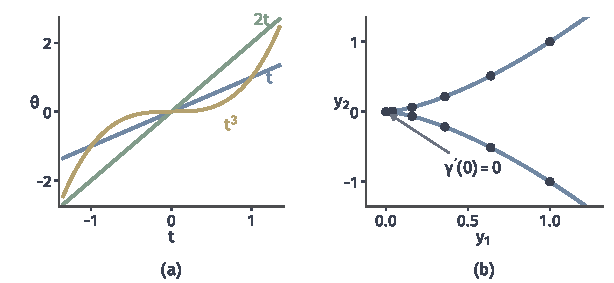
\includegraphics[width=104mm]{figures/04-spaces-measures-and-geometry/04-manifolds/matplotlib/mfd-curves-parametrization/figure.pdf}
  \caption{曲线是映射，不是点集。(a)圆周上三条曲线在角度图中的坐标曲线$\theta=t,2t,t^3$，三者经过相同的点，速度不同，$t^3$在$t=0$处速度为零。(b)平面曲线$\gamma(t)=(t^2,t^3)$的像，黑点是$t=-1,-0.8,\ldots,1$时的位置。分量都是多项式，映射光滑，像却在原点有尖点，那一刻速度恰好为零，黑点也在此处聚拢。}
  \label{fig:mfd-curves-parametrization}
\end{BookInlineFigure}

反过来，映射光滑，像却可以不光滑。平面曲线$\gamma(t)=(t^2,t^3)$的两个分量都是多项式，所以是光滑曲线。计算它的速度：
\[
\gamma'(t)=(2t,\ 3t^2),\qquad \gamma'(0)=(0,0).
\]
它的像$\{(y_1,y_2):y_1^3=y_2^2\}$在原点有尖点，见图~\ref{fig:mfd-curves-parametrization}(b)。尖点处速度恰好为零，所以光滑映射的像才可能在那里拐出尖角。因此“光滑曲线”说的是映射，不是点集；曲线的像能否成为一个光滑子流形，是第~\ref{chap:manifold-relations}章的问题。

\paragraph{边界点处的曲线}
在带边界流形中，曲线可以停在边界上，也可以从边界出发进入内部。闭圆盘中$\gamma(t)=(1-t,0)$，$t\in[0,1)$，从边界点$(1,0)$出发向内运动，只能取$t\geq0$；若取$t<0$，点会离开圆盘。所以过边界点的光滑曲线一般只能是单侧的。

下一节先在内点处用双侧曲线的速度建立切向量。边界点处只收集单侧曲线的速度，得到的是半个空间，而不是线性空间，那里的切空间要换一种方式定义，见第~\ref{sec:mfd-tangent-space}小节。
